%===================================== CHAP 5 =================================

\chapter{Experiments, Results and Discussion} \label{cap_5}


Chapter 3 discussed the different concepts regarding the pipeline and the examples data managed by it. Chapter 4 explained how the pipeline is implemented. In this chapter we will use the information made available in Chapter 3 and 4 and explore to which degree the research goals have been accomplished.\\
First, for Research Goal 1 we will decide whether the pipeline created is satisfactory or not. Regarding Research Goal 2, we will conclude the analysis conducted in Chapter 3. Next, we will investigate if the database chosen to manage the collection of examples is satisfying the purpose of Research Goal 3. Finally, a series of tests will be performed to measure the search results displayed by the search interface. A comparison of the results will help determine if Research Goal 4 is fulfilled. \\
Every section in Chapter 5 will discuss on of the research goals. Table \ref{table:rgSecMapping} gives a quick overview of which research goals are being discussed by the different sections.

\begin{table}[h]
\centering
\begin{tabular} {|| p{5em} | p{10em} ||} 
 \hline
  Goals & Section \\ [0.5ex] 
 \hline
1   &   \ref{5:pipeline} \\
2   &   \ref{5:example} \\
3   &   \ref{5:exampleCollection} \\
4   &   \ref{5:interface}, \ref{5:keywords} and \ref{5:queryByExample} \\
 \hline
\end{tabular}
\caption{Mapping of which sections discusses the different research goals.}
\label{table:rgSecMapping}
\end{table}

\section{Resulting Pipeline} \label{5:pipeline}

We tested the final pipeline by using the English Wikipedia's database dump from February 4. 2016. With a size of 56.3 GB, the XML file contains over five million articles. The process of extracting the relevant data and inserting it into the SQL database lasted nine hours. After the last section was added, the database contained 28 110 example sections deemed as relevant sections. The process was run on a mid end MacBook Pro from late 2013 with four cores, each with a processor speed of 2 GHz and 2x4 GB of memory with a speed of 1600 MHz.

When the process that extracts relevant sections were finished, a new fully independent process was started for the next step. First, the process queries the SQL database for sections\footnote{A section is a part of an Wikipedia article.}. By using the relations from the sections stored in the SQL database, the process builds examples. Next, a whitelist is used to filter the examples based on their categories. By filtering the examples we can avoid irrelevant categories, for instance examples concerning history. Finally, the collection of examples left are used to build an index with Elasticsearch. The Elasticsearch index offers an HTTP API that can be used to query for examples.


\begin{table}[H]
\centering
\begin{tabular} {|| p{15em} | r ||} 
 \hline
  & Value \\ [0.5ex] 
 \hline
XML file size in Gigabytes & 56.3 \\
Number of articles & ~5 100 000 \\
Extraction duration in hours & ~9 \\
CPU speed in GHz & 2.0 \\
Memory size in GB & 8 \\

 \hline
\end{tabular}
\caption{Results from processing the XML dump through the pipeline}
\label{table:run_statistics}
\end{table}


\section{Describing a good example} \label{5:example}
Finding examples that later can be presented to the user is the overall goal of our work. To make the system we have created perform well, we want to fill the database with useful data in the form of good examples. This project uses Wikipedia as a source to automatically identify and extract examples. To make the best out of the examples extracted, we performed an analysis on what differentiates a good example from a bad one. A more detailed account of the analysis can be found in section \ref{examples-section}. This section will use the main points from section \ref{examples-section} to draw a conclusion.

The analysis was performed based on examples from Wikipedia, but to compare examples for the same topic, examples from a normal Google search were also used. Game Theory is used as an overall domain for the analysis. The examples were chosen to walk through the unimplemented system. The analysis let us discover how the examples would affect the system, and depending on the system's input, the structure of the examples could be fitted to the system's needs.
The topics were chosen to reveal strengths and weaknesses of our approach. The following topics were chosen to find examples: Prisoners Dilemma, Nash Equilibrium, Pareto Optimality, Zero sum, Parrondos Paradox. Appendix \ref{app_example} contains samples of two examples chosen for the subject Pareto Optimality. 

Based on these subjects, a list of properties that examples might possess was compiled, table \ref{table:1} contains these properties with a short description of each. The properties listed in table \ref{table:1} are all favourable, but we experienced that when an example contains to many of them, the content of the example becomes very complex. A complex example is not necessarily a bad thing. Although a more complex example requires more prerequisite knowledge from the reader, which may exclude some readers. The extent of use for each property is also a considerable factor for determining complexity. Although more properties often make the content of the example more complicated, some are always needed. A simple example will have a hard time explaining the more complicated aspects of a subject. Therefor an example should fall in between a golden mean of complexity. This golden mean is hard to define, but ought to be quite large. There is some techniques though, that lets an example explain more complicated subjects, without increasing complexity. Pictures or equations that is methodically referenced to from a descriptive text, is one way. Also the combination of the properties analogies, walk-through and iterations improve examples without making them more complex. 

The analysis in section \ref{examples-section} gave a better understanding of examples. Consequently rating and ordering of examples can be improved based on the analysis. 
The improvement can result in the collection of examples having a higher quality and also lead to a better user experience. 


\section{Collection of examples} \label{5:exampleCollection}
Research Goal 3 aims to obtain a collection of examples that we can populate a database with. The database accepts all kinds of examples, consequently the examples are represented in a generic way. We are using Wikipedia as source for all the examples, therefor we have to strip away a large amount of the information from the articles used. 

After an article is extracted from the XML document, data is stored in a relational database. To form an example, data is fetched from the tables by using the relations defined in the SQL database. In addition to the content, categories and references associated with the example are included. These properties are needed for an example in our system, so we later can perform queries on the collection. With Wikipedia having no limits for its domains, whitelists are used to narrow the examples down into only relevant domains for our project. During implementation whitelist \textit{Top200Edu} and \textit{MathTechWiki} were used.

After the processing, the collection now contains relevant elements, with a structure that represents a general example. This collection can then be indexed by Elasticsearch, which is the database containing all examples. Other examples from different sources can separately be included to Elasticsearch's example index, as long as the examples are structured correctly according to the mapping described in section \ref{imp_indexer}. Table \ref{table_indexStats} shows how many examples that were extracted from Wikipedia and how many examples that ended up in the final index.


\begin{table}[H]
\centering
\begin{tabular} {|| p{15em} | r ||} 
 \hline
  & Value \\ [0.5ex] 
 \hline
Number of section after extraction & 28110 \\
Number of examples after filtering & 6593 \\
 \hline
\end{tabular}
\caption{Statistics from the index after original implementation.}
\label{table:indexStats}
\end{table}

\section{Search interface} \label{5:interface}

\begin{figure}[H] 
\caption{A screenshot of the search interface before a search is performed.}
\centering
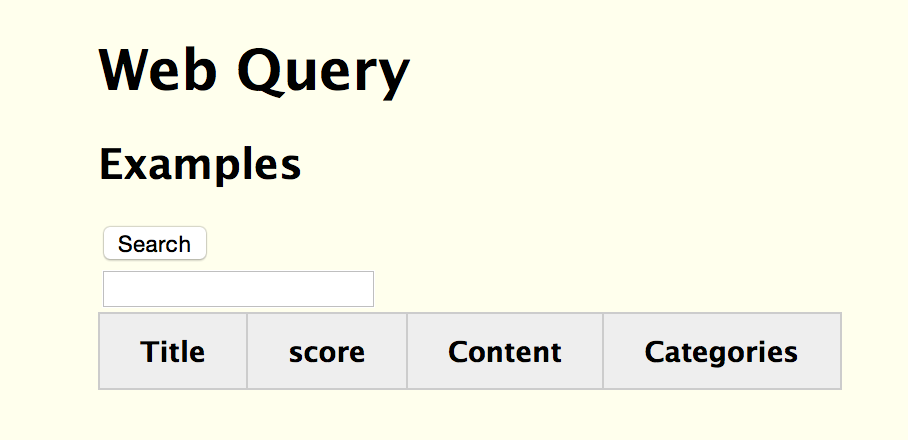
\includegraphics[scale=0.5]{wq_empty}
\label{fig:wq_empty}
\end{figure}

Figure \ref{fig:wq_empty} shows the search page of Example Search, before a search is performed. The design is very minimalistic with main focus on highlighting functionality. When a search is performed the now empty table will be filled with results. The columns \textit{Score} and \textit{Categories} are mainly for help to evaluate and debug the system by using the returned results.( Would not be necessary in a finished version.) Meanwhile \textit{Title} displays the name of the Wikipedia article and \textit{Content} contains the actual example.


\begin{figure}[H] 
\caption{A screenshot of the search interface after a search is performed, showing the returned results.}
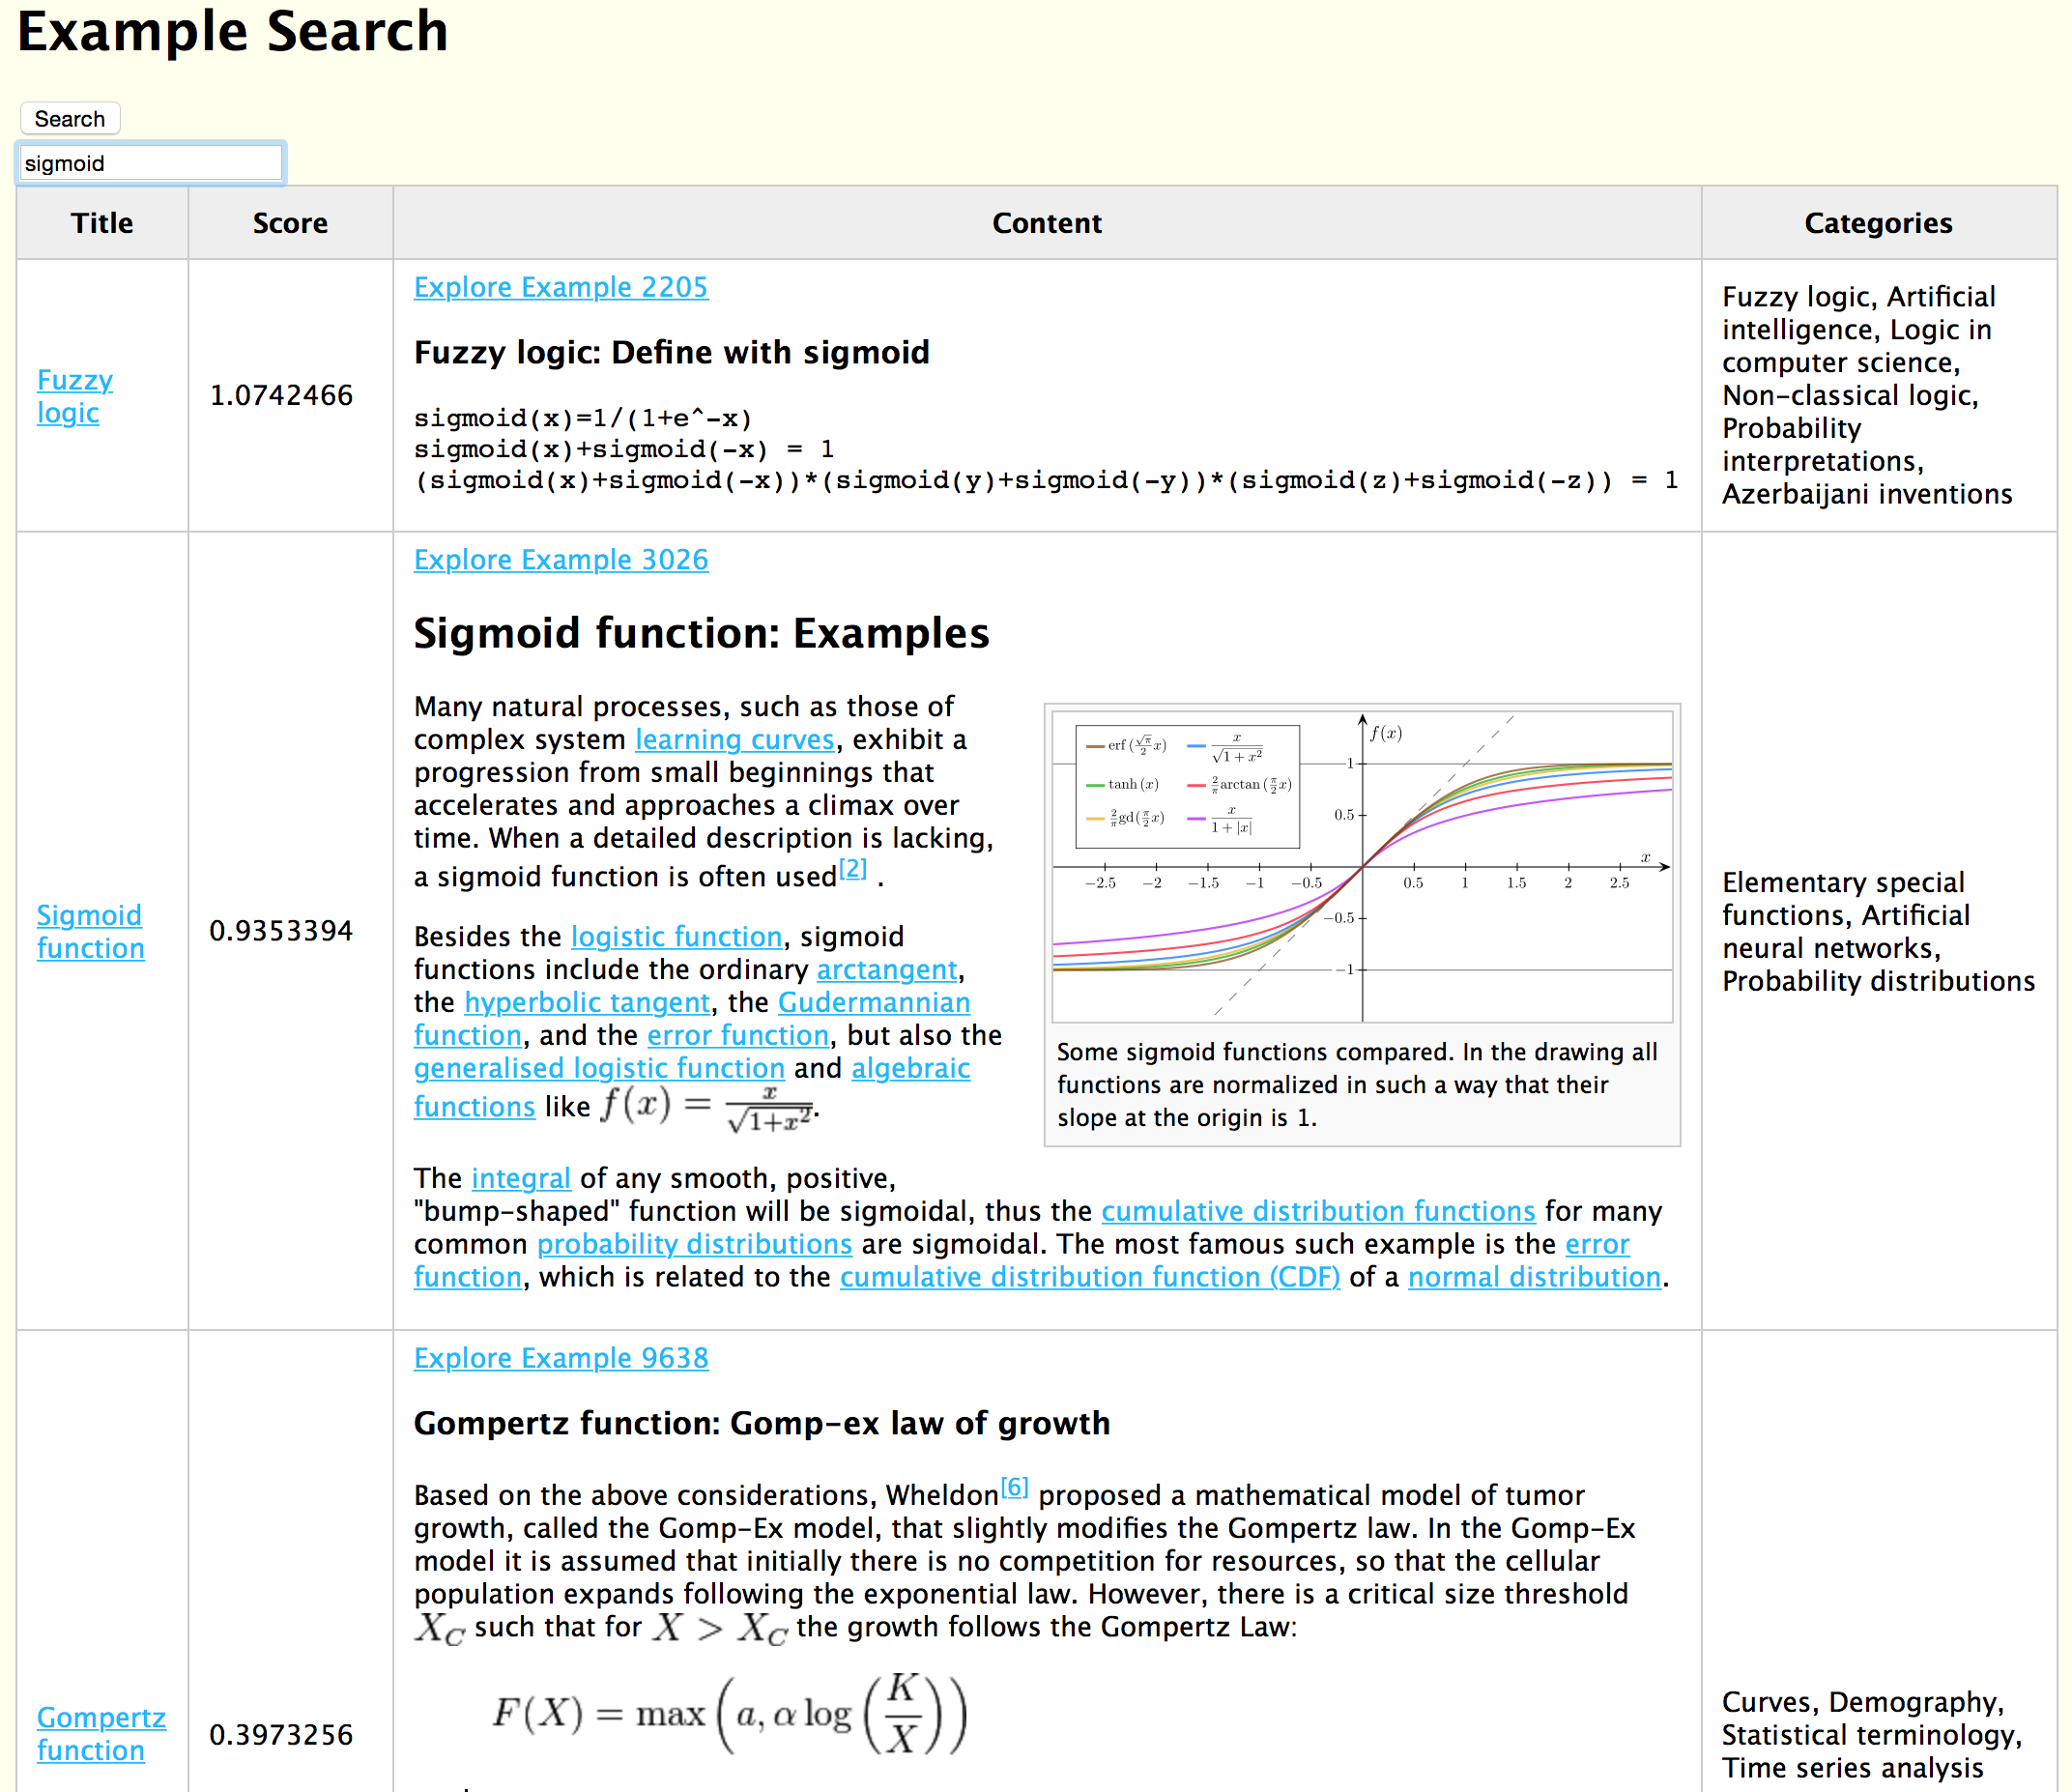
\includegraphics[width=\textwidth]{wq_results}
\label{fig:wq_results}
\end{figure}

When a search has been entered, the table expands and displays the examples returned. Figure \ref{fig:wq_results} demonstrates how the interface looks after the search term \textit{sigmoid} has been used. Every example has a link as its first line, which leads to a page specific for that example. When the link is clicked, the web server starts the process of finding related examples by sending a query to Elasticsearch and evaluating the returned results. The selected example and its related examples are then sent to the web page and displayed there.

This page can been seen in figure \ref{fig:wq_example}. The page has the main example displayed in the middle, while the columns at each side of it contains a list of related examples. The lists contains the name of examples and a link to their own page. The \textit{Total matches} list on the left side contains related examples with a total match, while on the right side is the \textit{Partial matches} list, which contains top ten of the examples that partly match. A search based on the category sets from the original search and the main example is used to find and order the relevant examples.

\begin{figure}[H] 
\caption{A screenshot of the search interface when a specific example has been chosen.}
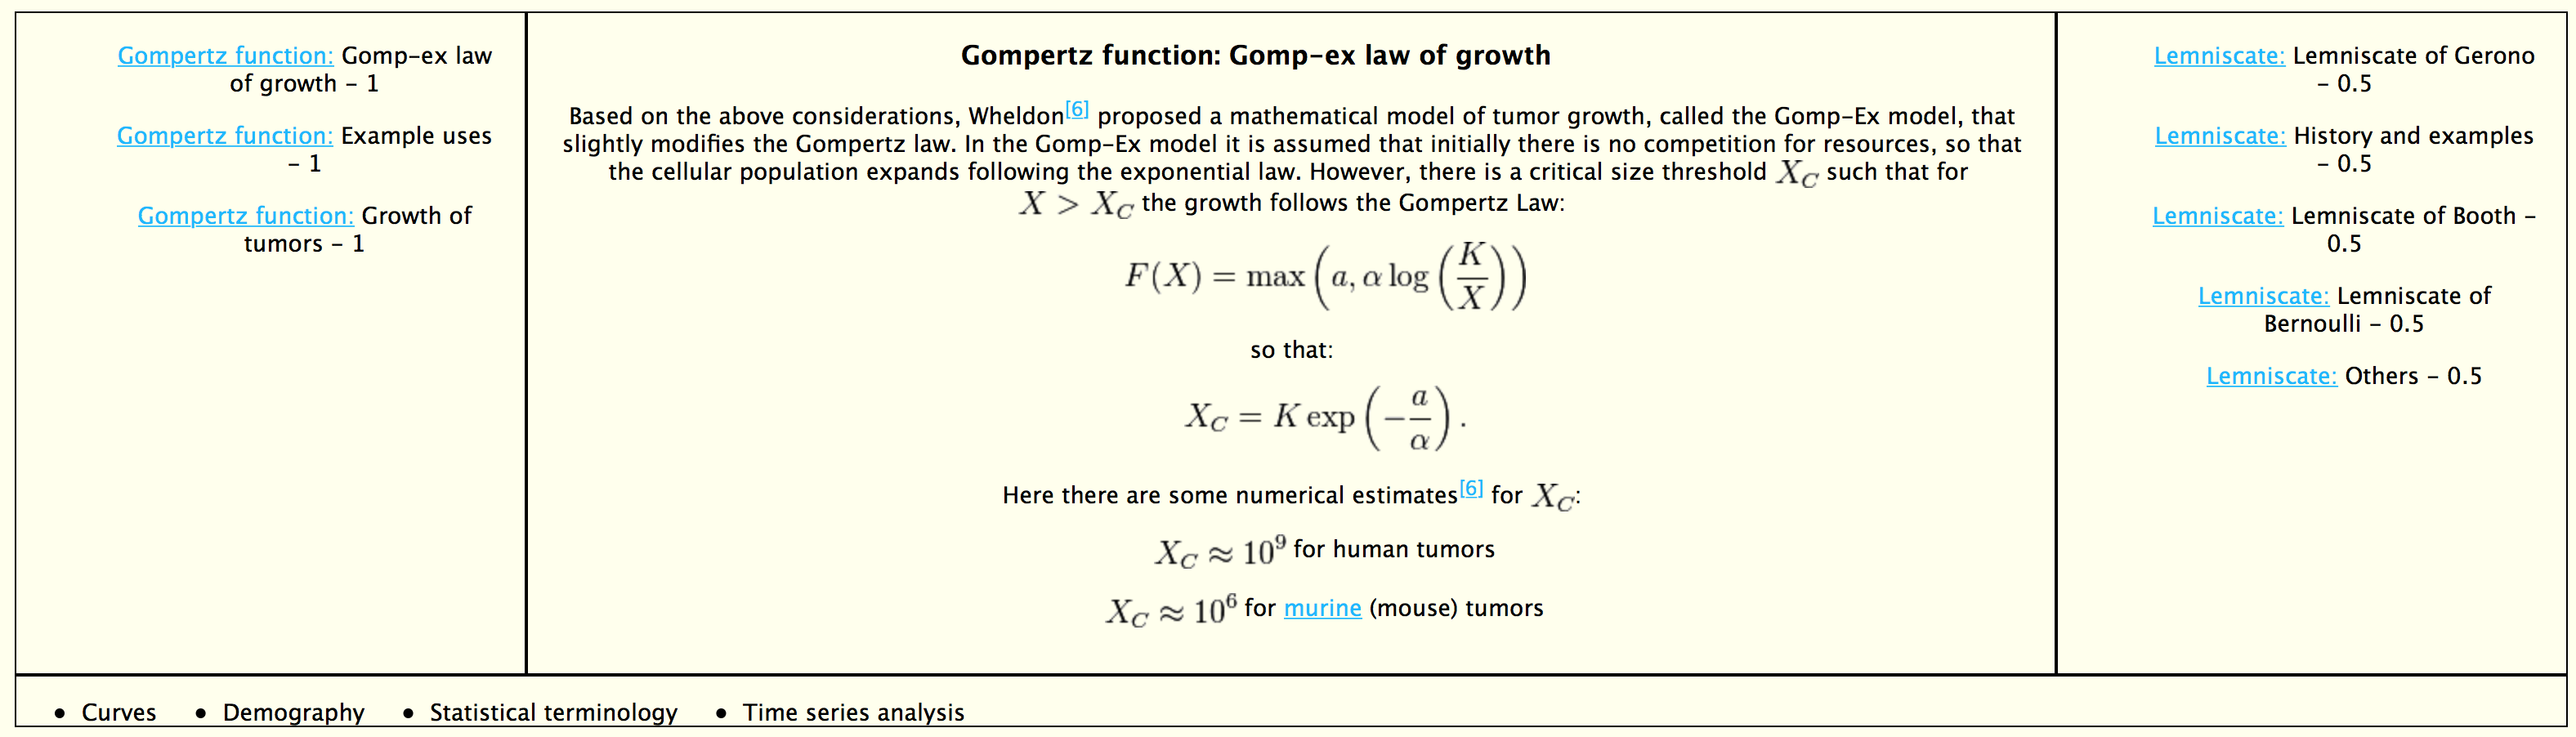
\includegraphics[width=\textwidth]{wq_example}
\label{fig:wq_example}
\end{figure}

\section{Querying by keywords} \label{5:keywords}

\subsection{Experiment I: Search examples} \label{search_experiment}
In this project we have filled a database with examples, indexed those examples and created a interface that we can use for searching them. In order to perform searches, we have created queries that Elasticsearch executes. To test how well these queries perform we have created a list of keywords. We test the accuracy of the queries by measuring the precision of the results returned from a search with the selected  keywords. Precision is the fraction of returned examples, which is relevant. It is calculated as follows:
\[\frac{|R \cap E |}{|E|}\]
In the equation above \(R\) is the set of all relevant examples and \(E\) is the set of all the retrieved examples.
In our experiments \(E\), representing all retrieved examples, is limited to the first five results in the top 5 tests, and similarly first ten in the top 10 tests. By limiting the size of \(E\), manual inspection can be used to check whether a example is actually relevant, which would also place it in the set \(R\).

%Precision is often used in combination with Recall, which is the fraction of relevant examples retrieved. Since we do not know how many relevant examples exist in total for each keyword, we can not measure recall. 


\begin{table}[h]
\centering
\small
\begin{tabular} {|| p{15em} | r | r | r ||} 
 \hline
 Keyword & Total hits & Top 5 & Top 10 \\ [0.5ex] 
 \hline

Logic & 362 & 1 & 0.9 \\
Programming & 884 & 1 & 0.9 \\
Heuristic & 44 & 0.8 & 0.7 \\
Algebra & 1046 & 0.8 & 0.7 \\
Game Theory & 2757 & 1 & 0.9 \\
\hline
Fuzzy Logic & 365 & 1 & 0.7 \\
Java & 269 & 1 & 0.9 \\
Bayes Network & 345 & 1 & 0.9 \\
Derivation & 67 & 1 & 0.8 \\
\hline
Chain Rule & 530 & 1 & 0.6 \\
Prisoners Dilemma & 39 & 1 & 0.6 \\
Nash Equilibrium & 101 & 1 & 0.8 \\
Cartesian Product & 789 & 0.8 & 0.6 \\
Parrondos Paradox & 49 & 0.6 & 0.4 \\
Zero Sum & 1017 & 0 & 0 \\

 \hline
\end{tabular}
\caption{The precision of the queries tested by a set of keywords and the top ten and top five results}
\label{table:precision_test}
\end{table}

Table \ref{table:precision_test} contains the keywords and the results of the test. The keywords were chosen from the domains mathematics, artificial intelligence and programming. Those retrieved examples that are faulty\footnote{Faulty examples can be caused by a bug in the pipeline or XML dump out of sync with the live Wikipedia page} or are examples for another subject are judged as an irrelevant result. Total hits reflects the amount of examples that the program found relevant to any degree. The different keywords have been divided into three different groups. The groups are ordered descending by the degree of how general the keyword is perceived. The horizontal line in the table separates the groups. There is no specific order among the keywords within a group.

\begin{figure}[H] 
\caption{Average precision for the three different groups}
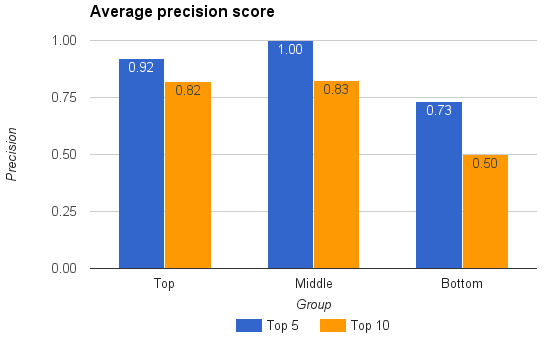
\includegraphics[width=\textwidth]{charts/ex1AvgPrec}
\label{fig:ex1AvgPrec}
\end{figure}

Figure \ref{fig:ex1AvgPrec} shows how the three different groupings score in the test. The top and middle group has a very good score, both for top 5 and top 10, while the bottom group score a bit lower. The average score of top 5 and top 10 for all three groups is \(0.8\), which entails that only 2 out of 10 examples are not relevant. This indicates that the system does a good job retrieving relevant examples.

The score in the top group for five and ten terms are very similar. In contrast the bottom group where the subjects are more specific, the score for top ten results suffers. Having a relatively small database of examples for specific topics is assumed to be the explanation. A richer selection of examples for the different topics could increase the precision for the bottom group. 

Another interesting remark to note is that the top 5 results are consistently better than the top 10 results. Top 5 being better than top 10, is caused by at least half of the relevant examples which is returned, are found among the first five results. Therefor we can conclude that the ranking of the examples functions as intended. 

There exist one substantial irregularity in table \ref{table:precision_test} though, the keyword \textit{Zero Sum} achieves a score of zero on both measures, meaning all of the ten first results returned is deemed irrelevant. No relevant results among the first ten could indicate an error in the system, either in the search itself, or that there is no example to find at all. 

While performing the experiment, the error occurred when searching with the keyword \textit{zero sum}. The system should have returned the example section from Wikipedia's article, \textit{Zero-sum game} \footnote{\url{https://en.wikipedia.org/wiki/Zero-sum\_game\#Example} (Last visited 28. April 2016)} as one of the examples in the result. An error analysis will help to determine why that did not happen, and in case of a system error, where in the system the error could have originated. 

To find the potential error we start at the beginning of the pipeline, to explore whether the example is retrieved from the XML dump. We find the answer in the SQL database. First we find a row in the \texttt{pages} table with the name \textit{zero sum game}. Next, using the primary key of this row, we can find all related rows in the table \texttt{page\_sections}. A query on the column \texttt{page\_id} in \texttt{page\_sections} returns one result. This result is the same section found in Wikipedia's article, thus we can conclude that Wikidump parser successfully inserts the section into the SQL database.

The next step is to verify that the section is transformed to an example and indexed by Elasticsearch. The examples in Elasticsearch shares the same id as the sections primary key in the SQL database. Querying Elasticsearch by id returns no results, therefor we know that the zero sum example never reaches Elasticsearch. Between the SQL database and Elasticsearch a whitelist filters the examples. If the zero-sum game article does not contain a category that exists in the whitelist, the example will be discarded. The article contains the categories \textit{Non-cooperative games} and \textit{International relations theory}. Matching the article's categories with the complete category list reveals that there exist only 4 occurrences of articles with Non-cooperative games as category and 7 with International relations theory, which is a low number. Whitelist \textit{Top200Edu} and \textit{MathTechWiki} were used for the filtering, section \ref{imp_indexer} explains whitelist's implementation and their function in our project. \textit{Top200Edu} includes only the top 200 relevant articles and \textit{MathTechWiki} use only the top level categories in the Wikipedia's category hierarchy. In conclusion, the article's categories is not included in any of the whitelists, and therefor the example is not indexed.

If the article's list of categories had been richer, the example would have been included more likely. Although richer category lists for Wikipedia's articles would have solved the problem, it is not something our project can affect. Instead a whitelist that accommodates the less popular categories is a better solution. The problem is that all the categories have to be manually added to whitelists. The Whitelist \textit{Edu} deals with the problem by including all categories, but also examining the most popular and removing the irrelevant categories from the whitelist. The disadvantage obtained by using \textit{Edu} is that irrelevant categories will be included, but on the other hand, they are not connected to many articles. 

\subsection{Experiment II: Whitelist}

The result of the error analysis in section \ref{search_experiment} points out the significance of the whitelists used for the end result. Based on that, Experiment II will be conducted to explore to what the degree the whitelists affect the results returned, and which of them is best to use. The tables used to display the result, will be identical to table \ref{table:precision_test} used in section \ref{search_experiment} with one exception. The tables in this section also include the percentage of hits compared to the number of examples in the index, when each specific whitelist has been applied. 

The first step in the experiment is to check what the system returns when there is no whitelists used. When no whitelists are used, there exist 28 110 examples in the index. Table \ref{table:p_test_no-list} shows the results.

\begin{table}[h]
\centering
\small
\begin{tabular} {|| p{10em} | r | r | r | r ||} 
 \hline
 Keyword & Total hits & \% of hits & Top 5 & Top 10 \\ [0.5ex] 
 \hline

Logic & 898 & 3.19 & 1 & 1 \\
Programming & 2135 & 7.60 & 0.8 & 0.9 \\
Heuristic & 81 & 0.29 & 1 & 0.8 \\
Algebra & 1629 & 5.80 & 1 & 0.9 \\
Game Theory & 6301 & 22.42 & 0.8 & 0.9 \\
\hline
Fuzzy Logic & 913 & 3.25 & 1 & 0.7 \\
Java & 523 & 1.86 & 0.8 & 0.9 \\
Bayes Network & 1370 & 4.87 & 0.8 & 0.9 \\
Derivation & 178 & 0.63 & 0.6 & 0.5 \\
\hline
Chain Rule & 1760 & 6.26 & 0.8 & 0.6 \\
Prisoners Dilemma & 141 & 0.50 & 0.8 & 0.5 \\
Nash Equilibrium & 350 & 1.25 & 1 & 1 \\
Cartesian Product & 2119 & 7.54 & 0.6 & 0.7 \\
Parrondos Paradox & 159 & 0.57 &  0.2 & 0.2 \\
Zero Sum & 2330 & 8.29 & 0 & 0.1 \\

 \hline
\end{tabular}
\caption{The precision of the queries tested when all examples are included.}
\label{table:p_test_no-list}
\end{table}
\clearpage

In the next step whitelist \textit{Edu} will be tested. \textit{Edu} contains most of the categories from the orignal category list, with the exception of categories that are popular, but not educational, being removed. A category's popularity is measured in how many examples links to the category. When the examples are filtered through \textit{Edu}, 5 133 examples are discarded from the original 28 110. The results of the test can be found in table \ref{table:p_test_list1}.

%%whitelist 1 : filtrert 5133 av 28110
\begin{table}[h]
\centering
\small
\begin{tabular} {|| p{10em} | r | r | r | r ||} 
 \hline
 Keyword & Total hits & \% of hits & Top 5 & Top 10 \\ [0.5ex] 
 \hline

Logic & 737 & 3.21 & 1 & 1 \\
Programming & 1783 & 7.76 & 0.8 & 0.9 \\
Heuristic & 72 & 0.31 & 1 & 0.8 \\
Algebra & 1337 & 5.82 & 1 & 0.8 \\
Game Theory & 5230 & 22.76 & 0.8 & 0.9 \\
\hline
Fuzzy Logic & 750 & 3.26 & 1 & 0.8 \\
Java & 442 & 1.92 & 0.8 & 0.9 \\
Bayes Network & 1171 & 5.10 & 0.8 & 0.9 \\
Derivation & 145 & 0.63 & 0.4 & 0.5 \\
\hline
Chain Rule & 1374 & 5.98 & 0.8 & 0.6 \\
Prisoners Dilemma & 115 & 0.50 & 0.8 & 0.5 \\
Nash Equilibrium & 60 & 0.26 & 1 & 1 \\
Cartesian Product & 1739 & 7.57 & 0.6 & 0.6 \\
Parrondos Paradox & 128 & 0.56 & 0.2 & 0.2 \\
Zero Sum & 1842 & 8.02 & 0 & 0.1 \\

 \hline
\end{tabular}
\caption{The precision of the queries tested when whitelist \textit{Edu} is used to filter the collection beforehand}
\label{table:p_test_list1}
\end{table}
\clearpage


The third test is conducted on whitelist \textit{Top200Edu}. \textit{Top200Edu} is similar to \textit{Edu} in terms of what type of categories are removed from the original list, with one big difference. \textit{Top200Edu} only keeps the 200 most popular categories, which means the educational categories which are not popular enough, are not included. Using \textit{Top200Edu} results in 21 746 examples being excluded from the index. Table \ref{table:p_test_list2} displays the results.


%%whitelist 2 : filtrert 21746 av 28110
\begin{table}[h]
\centering
\small
\begin{tabular} {|| p{10em} | r | r | r | r ||} 
 \hline
 Keyword & Total hits & \% of hits & Top 5 & Top 10 \\ [0.5ex] 
 \hline

Logic & 338 & 5.31 & 1 & 0.9 \\
Programming & 864 & 13.58 & 0.8 & 0.9 \\
Heuristic & 31 & 0.49 & 1 & 0.5 \\
Algebra & 1034 & 16.25 & 1 & 1 \\
Game Theory & 2701 & 42.44 & 0.8 & 0.8 \\
\hline
Fuzzy Logic & 341 & 5.36 & 0.8 & 0.5 \\
Java & 267 & 4.20 & 1 & 1 \\
Bayes Network & 315 & 4.96 & 1 & 0.9 \\
Derivation & 62 & 0.97 & 1 & 0.9 \\
\hline
Chain Rule & 515 & 8.09 & 1 & 0.6 \\
Prisoners Dilemma & 38 & 0.60 & 0.8 & 0.5 \\
Nash Equilibrium & 100 & 1.57 & 1 & 1 \\
Cartesian Product & 748 & 11.75 & 0.6 & 0.6 \\
Parrondos Paradox & 46 & 0.72 & 0.4 & 0.4 \\
Zero Sum & 1842 & 28.94 & 0 & 0 \\

 \hline
\end{tabular}
\caption{The precision of the queries tested when whitelist \textit{Top200Edu} is used to filter the collection beforehand}
\label{table:p_test_list2}
\end{table}
\clearpage

In the fourth step, we test whitelist \textit{MathTech}. \textit{MathTech} is based on \textit{Top200Edu}, but it narrows the domains of the categories deemed relevant to only concern Technology and Mathematics. \textit{MathTech} is a bit smaller than \textit{Top200Edu}, with 157 different categories. 23 073 examples are filtered out, when \textit{MathTech} is used. Table \ref{table:p_test_list3} reflects the results of the test.

%%whitelist 3: filtrert 23073 av 28110
\begin{table}[h]
\centering
\small
\begin{tabular} {|| p{10em} | r | r | r | r ||} 
 \hline
 Keyword & Total hits & \% of hits & Top 5 & Top 10 \\ [0.5ex] 
 \hline

Logic & 326 & 6.47 & 1 & 0.9 \\
Programming & 852 & 16.91 & 0.8 & 0.9 \\
Heuristic & 19 & 0.38 & 0.8 & 0.6 \\
Algebra & 991 & 19.67 & 1 & 1 \\
Game Theory & 2386 & 47.37 & 0.8 & 0.9 \\
\hline
Fuzzy Logic & 329 & 6.53 & 0.8 & 0.5 \\
Java & 265 & 5.26 & 1 & 1 \\
Bayes Network & 262 & 5.20 & 1 & 0.9 \\
Derivation & 56 & 1.11 & 1 & 1 \\
\hline
Chain Rule & 402 & 7.98 & 1 & 0.6 \\
Prisoners Dilemma & 33 & 0.66 & 0.8 & 0.5 \\
Nash Equilibrium & 87 & 1.73 & 1 & 1 \\
Cartesian Product & 606 & 12.03 & 0.6 & 0.6 \\
Parrondos Paradox & 37 & 0.73 & 0.4 & 0.4 \\
Zero Sum & 917 & 18.21 & 0 & 0 \\

 \hline
\end{tabular}
\caption{The precision of the queries tested when whitelist \textit{MathTech} is used to filter the collection beforehand}
\label{table:p_test_list3}
\end{table}
\clearpage

In the final step we test the most conservative whitelist, \textit{MathTechWiki}. \textit{MathTechWiki} is based on Wikipedia's category hierarchy, were Mathematics, Logic, Mathematical Sciences, Computing and their sub categories have been included. Applying \textit{MathTechWiki} leads to the removal of 27 107 examples. Table \ref{table:p_test_list4} contains the results of the final test. 

%%whitelist 4: filtrert 27107 av 28110
\begin{table}[h]
\centering
\small
\begin{tabular} {|| p{10em} | r | r | r | r ||} 
 \hline
 Keyword & Total hits & \% of hits & Top 5 & Top 10 \\ [0.5ex] 
 \hline

Logic & 100 & 9.97 & 1 & 1 \\
Programming & 107 & 10.67 & 0.2 & 0.3 \\
Heuristic & 20 & 1.99 & 0.6 & 0.4 \\
Algebra & 165 & 16.45 & 0.8 & 0.6 \\
Game Theory & 476 & 47.46 & 0.8 & 0.8 \\
\hline
Fuzzy Logic & 101 & 10.07 & 1 & 0.6 \\
Java & 9 & 0.90 & 0.4 & 3/9 \\
Bayes Network & 102 & 10.17 & 0.8 & 0.6 \\
Derivation & 22 & 2.19 & 0.6 & 0.4 \\
\hline
Chain Rule & 120 & 11.96 & 0.2 & 0.1 \\
Prisoners Dilemma & 8 & 0.80 & 0.4 & 2/8 \\
Nash Equilibrium & 17 & 1.69 & 1 & 0.9 \\
Cartesian Product & 126 & 12.56 & 0 & 0.1 \\
Parrondos Paradox & 18 & 1.79 & 0 & 0 \\
Zero Sum & 169 & 16.85 & 0.2 & 0.1 \\

 \hline
\end{tabular}
\caption{The precision of the queries tested when whitelist \textit{MathTechWiki} is used to filter the collection beforehand}
\label{table:p_test_list4}
\end{table}
\clearpage



\subsection{Discussion of results}



Figure \ref{fig:avgPrecision} shows the average precision for each whitelist. It gives an overview of how the different whit lists performed during Experiment II, making a comparison between them easy. While the score for top 10 has a very low deviation, \textit{Top200Edu} and \textit{MathTech} separates themselves from the rest for the top 5 measure. This indicates that keeping the most popular 200 categories can work well as a general strategy. The rest of this section will discuss different observations made during and after the experiment. To discuss the observations charts showing the results of different queries will be referenced, see appendix \ref{a:ex2} for charts related to keywords not mentioned in this section.

\begin{figure}[H] 
\caption{Average precision for all whitelists}
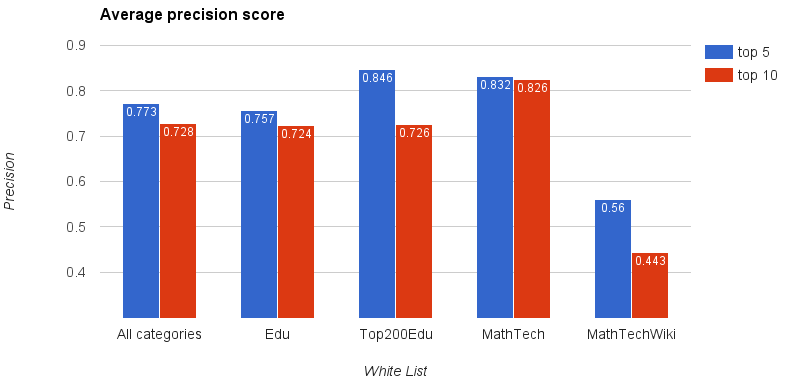
\includegraphics[width=\textwidth]{charts/avgPrecision}
\label{fig:avgPrecision}
\end{figure}

\begin{figure}[h] 
\caption{Precision score when the keyword \textit{Zero Sum} is used as a search phrase, with the different whitelists applied.}
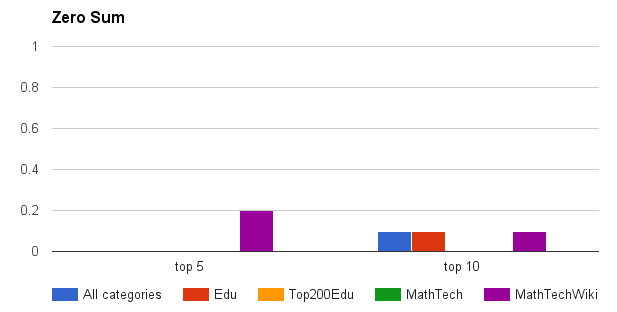
\includegraphics[width=\textwidth]{charts/zs}
\label{fig:zs}
\end{figure}

\paragraph{Lack of relevant results}
Figure \ref{fig:zs} displays the results when all the different whitelists have been applied when the keyword \textit{zero sum} has been used as search phrase. All the whitelists have very low precision, either zero results or only one among the top ten. Although the results are inadequate, they do contradict the claim in section \ref{search_experiment}'s error analysis, which suspected that no Zero Sum examples existed in the collection. Section \ref{search_experiment} drew that conclusion because the main article about Zero sum was not included in the collection. When only \textit{MathTechWiki} were tested, one relevant example was returned. This leads us to believe the abnormality was caused by using a bad combination of whitelists, making the other example not appearing among the top ten. The more thorough tests in experiment II, also points to the query not handling the keyword as a search phrase very well. In conclusion, the combination of faulty whitelist union and poor handling of the search phrase, are the reasons for the Zero sum's complete lack of relevant results in Experiment I.

\begin{figure}[h] 
\caption{Precision score when the keyword \textit{Java} is used as a search phrase, with the different whitelists applied.}
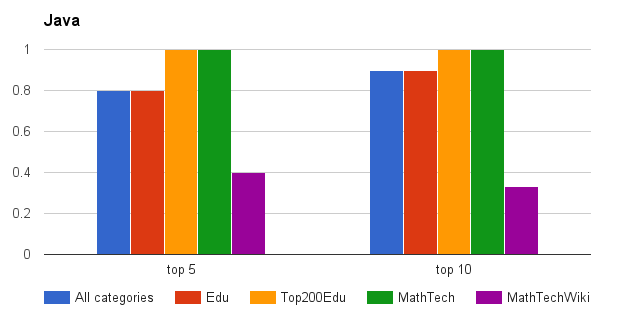
\includegraphics[width=\textwidth]{charts/j}
\label{fig:j}
\end{figure}

\paragraph{Few returned documents}
In table \ref{table:p_test_list4} we note that many of the keywords have very few total hits. In particular, the keywords \textit{java} and \textit{prisoners dilemma} returns less than 10 results, making the top 10 test inaccurate. Having so few total hits is reflected in the precision also dropping quite low. In figure \ref{fig:avgPrecision} we can see that the whitelist \textit{MathTechWiki} separates itself from the rest of the lists with almost 50 percent worse precision. This big loss of precision indicates that the whitelist excludes to many relevant examples from the index's corpus. Figure \ref{fig:j} demonstrates how the keyword \textit{java} overall has extremely good results, but when \textit{MathTechWiki} is applied, the score drops significantly lower.

\begin{figure}[h] 
\caption{Precision score when the keyword \textit{Derivation} is used as a search phrase, with the different whitelists applied.}
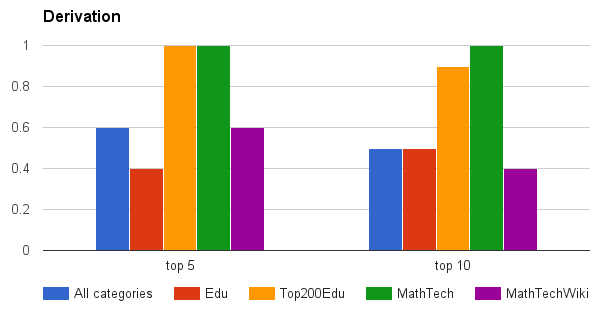
\includegraphics[width=\textwidth]{charts/d}
\label{fig:d}
\end{figure}

\paragraph{Excluding irrelevant examples}
Whitelists were used to exclude irrelevant examples by focusing on a particular domain. There is though a golden middle ground of how inclusive the whitelist should be. The whitelists \textit{Top200Edu} and \textit{MathTech} seems to have more or less the right amount of inclusiveness. In Figure \ref{fig:avgPrecision}, they have the best average score for the top 5 results, and they are equal with \textit{Edu} regarding top 10. When the keyword \textit{derivation} was tested, \textit{Top200Edu} and \textit{MathTech} accomplished a perfect score, except for one irrelevant result among top 10 for \textit{Top200Edu}. Figure \ref{fig:d} shows how the score is significantly better than when the other lists were tested. The results returned explains the big difference. A lot of results related to language and the word \textit{derive}, lead to many irrelevant examples. Since \textit{Top200Edu} and \textit{MathTech} are much stricter whitelists, those irrelevant examples was not a part of the index's corpus.

\paragraph{Multiple words in search phrase}
While discussing the results from keyword \textit{zero sum}, poor handling of the keyword, was a part of the conclusion. The poor handling is experienced by highly unrelated examples being returned after a search. \textit{Zero sum} demonstrates the most extreme side of the issue, but similar behaviour exists for other keywords also. The problem occur because the keyword uses two words. Elasticsearch will then split the keyword into two search terms, and will not prioritize or reward examples who contains the those two words directly next to each other. The rarity of the words also has a big part to play. For instance \textit{nash equilibrium} also contains two words, but both are pretty rare. "Nash" is never used without being accompanied by "equilibrium". Although "equilibrium" exist in some examples which are not related to Nash Equilibrium, they are very few. Some keywords have one rare word and one common, for instance \textit{prisoners dilemma} and \textit{cartesian product}. These keywords achieve a mediocre result, with an average precision around 0.6. When considering the effects rarity of the word causes for keywords containing two words, it makes sense that \textit{zero sum}, which has two common words, have such a low precision. 

Order and proximity of the words are not a new problem in the field of information retrieval. Boosting the score of results based on how close the words appear, and if in right order, is a common technique. It could be done for this system, but it might end up being a to complicated solution, for an pretty straightforward problem. A simpler solution is to surround the words with quotation marks. The quotation marks will tell the index to handle all words between the quotation marks as a single search term. Since users often will search after name of examples or subjects, it will be enough to only accept examples where the terms are directly next to each other when the quotation mark surrounds the keyword.

\paragraph{Union of whitelists}
In Experiment II, the union of two whitelists were used, \textit{Top200Edu} and \textit{MathTechWiki}. This union gave the average score of \(0.8\), none of the whitelists in Experiment II matched this score, \textit{MathTech} was closest with \(0.76\). Although this whitelist union gave better results than any independent whitelist, it showed weaknesses for other cases, in particular the case of no results for \textit{zero sum}, and \textit{algebra} achieving a perfect precision for \textit{MathTech}. With that in mind, a new union of whitelists should be formed, that also could handle edge cases, either by finding a new combination or creating new whitelists.


\section{Querying by examples} \label{5:queryByExample}

\subsection{Experiment III: Finding related examples}

When querying by examples, relevant examples that assists in learning of the subject, are expected to be returned. To evaluate how the system accomplishes this, we will make us of observations from section \ref{5:keywords}. The observations will be used to create an optimal environment, by choosing the best performing whitelist and a keyword with perfect precision. The whitelist \textit{MathTech} performed best for the top ten results with an average precision of 0.72, and will therefor be the whitelist chosen. As keyword, \textit{Java} will be used for mainly three reasons. First, it is on of the keywords with a perfect score when \textit{MathTech} was applied as whitelist. Second, \textit{java} is a search phrase, but at the same time not the exact name of a category. Finally, it is very easy to consistently judge whether an example is about java or not, since it often contains java code. For an example to be deemed relevant, it will be satisfactory for the example to be an example within the Java domain. 

When testing there are three numbers that will be considered for the assessment of the system's performance. First, how many examples are shown together with the main example. Second, how many of the examples are relevant. In addition, the number of the main example's categories will be included, to explore a possible correlation. The first ten examples will be used in the test. The results will be divided between the right and the left list.

\begin{table}[H]
\centering
\small
\begin{tabular} {|| r | r | r | r | r | r ||} 
\hline
 & \multicolumn{2}{ c |}{Total matches} & \multicolumn{2}{ c |}{Partial matches} &  \\

Example & Total & Relevant & Total & Relevant & Categories\\ [0.5ex] 
\hline

1	&	2	&	2	&	10	&	10	&	3	\\
2	&	2	&	2	&	10	&	10	&	3	\\
3	&	2	&	2	&	10	&	10	&	6	\\
4	&	2	&	2	&	10	&	10	&	3	\\
5	&	4	&	4	&	10	&	10	&	5	\\
6	&	4	&	4	&	10	&	10	&	5	\\
7	&	0	&	0	&	10	&	10	&	3	\\
8	&	27	&	27	&	10	&	10	&	6	\\
9	&	2	&	2	&	10	&	10	&	6	\\
10	&	3	&	3	&	10	&	10	&	2	\\

\hline
\end{tabular}
\caption{Statistics for the test of querying by examples with \textit{java} as keyword}
\label{table:qbe_java}
\end{table}

The first column of table \ref{table:qbe_java} represents an example, with the number being its order among the returned examples after the search. The next column shows total number of examples and how many of them that are relevant, both for the lists at the left and the right side. The last column shows how many categories the example have.

A quick look at the results presented in table \ref{table:qbe_java}, reveals consistently good results. To verify whether the performance of the system is as good as the results tell or if Java is a special case, a second test will be performed. The keyword \textit{nash equilibrium} is chosen, based on the same reason as why \textit{java} was chosen. There is one important difference that might make an impact. Java is a more general subject and therefor has \textit{java} 265 total hits, meanwhile the more specific \textit{nash equilbrium} has 87 total hits. In the second test, all examples discussing or referencing to a Nash Equilibrium related to the example's topic, will be deemed relevant.

\begin{table}[H]
\centering
\small
\begin{tabular} {|| r | r | r | r | r | r ||} 
\hline
 & \multicolumn{2}{ c |}{Total matches} & \multicolumn{2}{ c |}{Partial matches} &  \\

Example & Total & Relevant & Total & Relevant & Categories\\ [0.5ex] 
\hline

1	&	6	&	6	&	9	&	3	&	4	\\
2	&	6	&	6	&	9	&	3	&	4	\\
3	&	6	&	6	&	9	&	3	&	4	\\
4	&	6	&	6	&	9	&	3	&	4	\\
5	&	72	&	29	&	0	&	0	&	1	\\
6	&	72	&	29	&	0	&	0	&	1	\\
7	&	72	&	29	&	0	&	0	&	1	\\
8	&	6	&	6	&	9	&	3	&	4	\\
9	&	0	&	0	&	10	&	5	&	3	\\
10	&	6	&	6	&	9	&	3	&	4	\\

\hline
\end{tabular}
\caption{Statistics for the test of querying by examples with \textit{nash equilibrium} as keyword}
\label{table:qbe_ne}
\end{table}

\subsection{Discussion of results}

After conducting the second test, a big variation in the quality of results occurred compared to the first test. Despite the numbers differing, one pattern emerged in both tests. In table \ref{table:qbe_java} example 1, 2 and 4 have the pattern, and 1, 2, 3, 4, 8 and 10 in \ref{table:qbe_ne}. For these examples, the numbers are completely identical. They are identical because they come from the same article. Many Wikipedia articles have several example sections, which are used to explain the subject. Several examples originating from the same article not only results in them all achieving very similar score after a keyword search, but they will also have exactly the same categories. 

A similar pattern emerges between example 5, 6 and 7 in table \ref{table:qbe_ne}. The difference in this case is that the examples all originate from different articles. The reason they still achieve the same results is because they all have the same set of categories in common, since the algorithm used to find and measure related examples solely uses categories. In this case only one category, \textit{game theory}. Only \textbf{one} category is also what is causing the big difference between the left and the right list. All the examples achieving a perfect match with the selected example, only need to have Game Theory as a category. This leads to related examples either having a total match or none match at all, with few of the examples having a total match being related. A solution could either be connecting more categories to the examples or create a better version of the matching algorithm.  

There is some positive patterns that can be noticed to. For instance, all the related examples returned for the keyword \textit{java} is also relevant. One of the things that causes this is already explained, being many examples originating from the same article. Another factor causing the high degree of relevance is the observation that many of the examples is included in a considerable amount of the lists. A big portion of the examples were also a part of the initial search's results. These remarks points towards the system showing a good tendency regarding finding related examples.


\cleardoublepage